\section{Introduzione}

\subsection{Parte di back-end}

\subsubsection{Database}\label{Database}

\paragraph{Introduzione}
Tenendo conto dei requisiti e dell’archittettura da rispettare del capitolato, si sono sviluppati 2 database: “issuerdb” per l’Issuer e “walletdb”  per lo User (cioè l’utente in possesso del proprio portafoglio digitale).

\paragraph{Issuerdb}
    
\begin{center}
    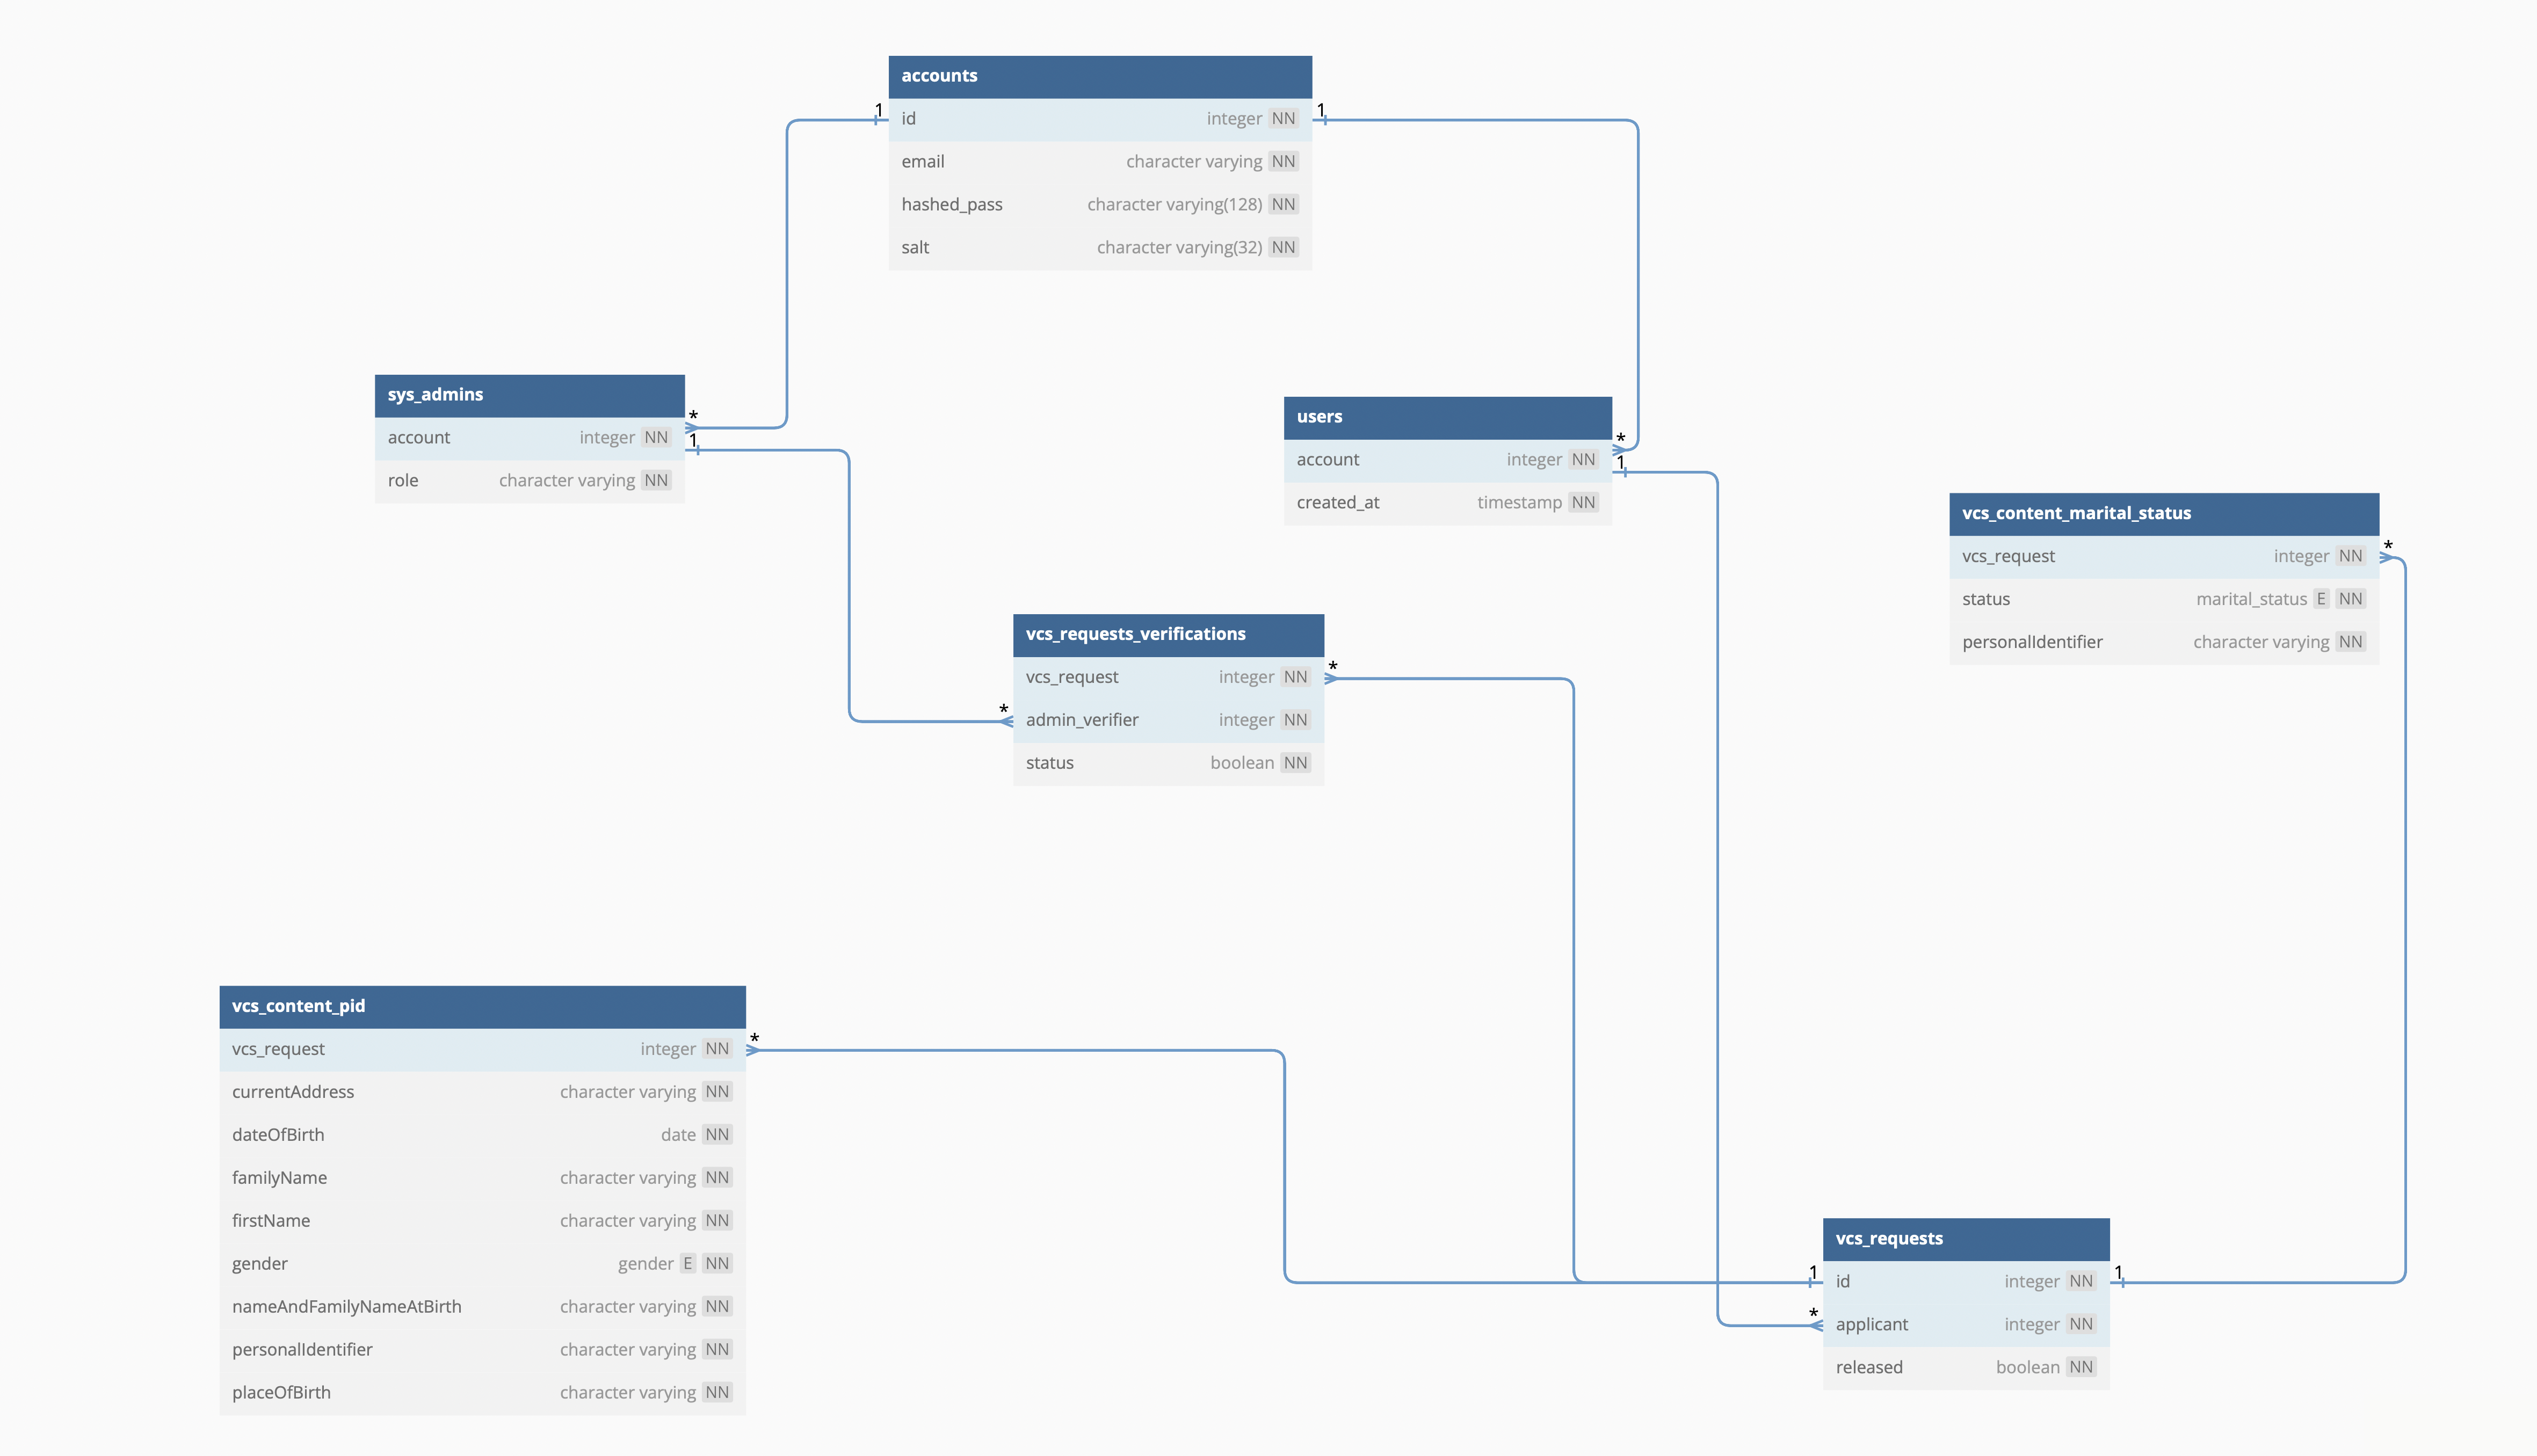
\includegraphics[scale = 0.9]{./res/img/issuerdb.png}
  \end{center}
L'immagine sopra riportata descrive il database "issuerdb" implementato mediante un grafico entità-relazioni (schema ER).\\
Issuerdb è stato pensato per gestire e conservare le informazioni legate agli utenti, alle richieste di certificati digitali (VCS requests) e alle verifiche dei certificati stessi.
Per quanto richiesto dal capitolato, e per rispettare la logica dietro tutto il meccanismo dell'Issuer, si distinguono 2 tipi diversi di account: gli account "sys\_admins" e gli account "users".\\
\begin{itemize}
\item "sys\_admins" sono gli account utilizzati dagli amministratori di sistema, cioè quelle entità che si occupano di approvare (o meglio, verificare) le richieste degli "users" (VCS requests).\\
\item "users", invece, sono gli account utilizzati dai semplici utilizzatori del servizio. Si occupano semplicemente di effettuare delle richieste di certificati di loro interesse alle entità che si occupano di verificare i certificati.\\
\end{itemize}
Il contenuto della richiesta approvata e rilasciata può essere di 2 tipi soltanto: un "vcs\_content\_marital\_status" (contenuto riferito allo stato di matrimonio di un utente) o un "vcs\_content\_pid" (contenuto riferito ad un documento PID di un utente).\\
Più in dettaglio:\\\\
\textbf{Tipi enumerati}: sono definite due tabelle ENUM per rappresentare:
\begin{itemize}
    \item il genere maschile/femminile (“gender”, che può avere come valori “M” o “F”);
    \item lo stato civile (“marital\_status”, che può avere come valori “married”, “cohabitant”, “divorced”,”widower”, “separate”, “canceled”, “other”).
\end{itemize}
Queste tabelle verranno utilizzate per definire, rispettivamente, gli attributi “gender” della tabella “vcs\_content\_pid” e “marital\_status” della tabella “vcs\_content\_marital\_status”.\\\\

\textbf{Tabella “accounts”}:
\begin{itemize}
    \item “id”: identificativo univoco per l’account, chiave primaria; 
    \item “email”: indirizzo email dell’account, varchar not null;
    \item “hashed\_pass”: password hash dell’account, varchar massimo 60 caratteri not null;
    \item “salt”: salt usato per la sicurezza nella creazione dell’hash della password dell’account dell’utente, varchar massimo 22 caratteri not null.
\end{itemize}

\textbf{Tabella “users”}:
\begin{itemize}
    \item “account”: riferimento all'id della tabella "accounts", identificativo univoco per l’account degli utilizzatori,  chiave primaria;
    \item “created\_at”: data di creazione dell’account, formato timestamp not null. 
\end{itemize}

\textbf{Tabella “sys\_admins”}:
\begin{itemize}
    \item “account”: riferimento all'id della tabella "accounts", identificativo univoco per l’account degli amministratori,  chiave primaria; 
    \item “role”: ruolo dell'amministratore di sistema, varchar not null.
\end{itemize}

\textbf{Tabella “vcs\_requests”}:
\begin{itemize}
    \item “id”: identificativo univoco della richiesta del certificato; 
    \item “applicant”: riferimento all'account dell'utente nella tabella "users", integer not null;  
    \item “released”: flag per indicare se il certificato è stato rilasciato, variabile booleana not null. 
\end{itemize}

\textbf{Tabella “vcs\_requests\_verifications”}:
\begin{itemize}
    \item “vcs\_request”: riferimento all'id di una richiesta nella tabella "vcs\_requests";  
    \item “admin\_verifier”: riferimento all'account dell'amministratore di sistema;  
    \item “status”: stato della verifica, variabile booleana not null. 
\end{itemize}

\textbf{Tabella “vcs\_content\_pid”}:
\begin{itemize}
    \item “vcs\_request”: riferimento all'identificativo di una richiesta nella tabella "vcs\_requests" e “vcs\_requests\_verifications”; 
    \item “currentAddress”: l’indirizzo corrente scritto nel documento PID, varchar not null; 
    \item “dateOfBirth”: data di nascita scritta nel documento PID, varchar not null;  
    \item “familyName”: cognome scritto nel documento PID, varchar not null; 
    \item “firstName”: nome scritto nel documento PID, varchar not null; 
    \item “gender”: genere scritto nel documento PID, enum con valori “M”/”F” not null; 
    \item “identifier”: identificatore scritto nel documento PID, varchar not null; 
    \item “nameAndFamilyNameAtBirth”: nome e cognome di famiglia scritto nel documento PID, varchar not null;
    \item “personalIdentifier”: identificatore personale scritto nel documento PID, varchar not null.
\end{itemize}

\textbf{Tabella “vcs\_content\_marital\_status”}:
\begin{itemize}
    \item “vcs\_request”: riferimento all'identificativo di una richiesta nella tabella "vcs\_requests" e “vcs\_requests\_verifications”; 
    \item “status”: stato civile = stato di matrimonio, enum corrispondente ai valori della tabella “marital\_status”, not null;  
    \item “personalIdentifier”: identificatore personale per es. codice fiscale, varchar not null.
\end{itemize}


\textbf{RELAZIONI FRA LE TABELLE}
\begin{itemize}
    \item \textbf{“accounts” – “sys\_admins” e “users”}: “accounts” – “sys\_admins” e “accounts” – “users” relazione 1-1. Un account appartiene a un solo utente, un utente può avere soltanto un account. Un account appartiene a un solo amministratore, un amministratore può avere solo un account. Un account è un account “sys\_admins” oppure un account “users”, non può essere entrambi. La relazione deve essere unica, e questo limite si controlla nel back-end (poiché nel database non c’è modo di controllare l’unicità della relazione). Nel back-end si controllerà anche se un account è sia un account amministratore che un account user (con conseguente errore).
    \item \textbf{“sys\_admins” – “vcs\_requests\_verifications”}: relazione 1-N. Una verifica di richiesta appartiene al massimo ad un amministratore. Un amministratore può verificare molteplici richieste.
    \item \textbf{“users” – “vcs\_requests”}: relazione 1-N. Una richiesta di credenziale può appartenere al massimo ad un user. Un user può fare molteplici richieste.
    \item \textbf{“vcs\_requests\_verifications” e “vcs\_requests” – “vcs\_content\_marital\_status” e “vcs\_content\_pid”}: similmente a prima, il contenuto del VCS o è un contenuto relativo al “marital status”, oppure un contenuto relativo al “PID” (non entrambi, ma deve essere obbligatoriamente un contenuto di marital status oppure un contenuto di PID). Questa condizione sarà controllata nel back-end. La richiesta sarà rilasciata DOPO che la richiesta sarà approvata dal verificatore. Per essere rilasciata (dopo essere approvata), l’utente riceve la richiesta come credenziale (con conseguente stoccaggio nel “walletdb”). Una volta ricevuta, la richiesta verrà contrassegnata come “true” (nel campo “released” in “vcs\_requests”). Invece, il campo “status” in “vcs\_requests\_verifications” indica se la richiesta è stata approvata dal verificatore. Se lo “status” sarà “true”, allora la richiesta sarà pronta per il rilascio (quindi lo status “true” dell’attributo “released” di “vcs\_requests” dipende dallo status “true” dell’attributo “status” di “vcs\_requests\_verifications”). Una richiesta può essere verificata una sola volta. Una verifica appartiene ad una e una sola richiesta. Se la richiesta non è stata ancora approvata non si può richiedere una riapprovazione. Se la richiesta è stata verificata con esito status=”false” soltanto allora si può fare un altro tentativo di richiesta. Per questo motivo la relazione fra “vcs\_requests” e “vcs\_requests\_verifications” è 1-1.
\end{itemize}



\paragraph{Walletdb}
\begin{center}
    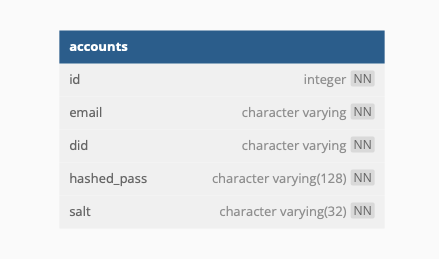
\includegraphics[scale = 0.3]{./res/img/walletdb.png}
  \end{center}

L’immagine sopra riportata descrive il database “walletdb” implementato mediante un grafico entità-relazioni (schema ER).
Walletdb è stato pensato per gestire e conservare (fare lo “storing”) le informazioni legate alle credenziali degli utenti, come espresso da capitolato.\\
Più in dettaglio:\\\\
\textbf{Tabella “accounts”}:
\begin{itemize}
    \item "id": identificativo univoco per l'account degli utenti, chiave primaria,
    \item "email": indirizzo email associato all'account, varchar not null,
    \item "did": documento did associato all'account dell'utente, varchar,
    \item "hashed\_pass": password hash dell'account dell'utente, varchar massimo 60 caratteri not null,
    \item "salt": salt usato per la sicurezza nella creazione dell'hash della password dell'account dell'utente, varchar massimo 22 caratteri not null,
    \item “created\_at”: data di creazione dell’account, timestamp not null.
\end{itemize}
\subsection{Parte di front-end}


\subsection{Componente di API}


\subsection{Design pattern}